\documentclass[a4paper]{scrartcl}

\usepackage[T1]{fontenc}

\usepackage{amsmath,amssymb}

\usepackage[square, comma, numbers, sort&compress]{natbib}

\usepackage{tikz}

\usepackage[pdftex, colorlinks]{hyperref}
\usepackage[figure, table]{hypcap} % Fix a problem with hyperref
\hypersetup{
    bookmarksnumbered,
    pdfstartview={Fit},
    citecolor={black},
    linkcolor={black},
    urlcolor={black},
    pdfpagemode={UseOutlines}
}

% Make hyperlinks jump to the right place
\makeatletter
\newcommand\org@hypertarget{}
\let\org@hypertarget\hypertarget
\renewcommand\hypertarget[2]{%
\Hy@raisedlink{\org@hypertarget{#1}{}}#2%
} \makeatother

% Space between paragraphs, rather than indented paragraphs
\parindent 0pt
\parskip 1ex

% Bibliography style
%\bibliographystyle{unsrtnat} % `Plain' unsrtnat.bst
\bibliographystyle{ajbunsrtnat} % Modified unsrtnat.bst to make article titles emphasized

\title{Computing Course Day 5\\
Notes \& Discussion\\
Second Edition}
\author{Andrew J. Bennieston}
\date{\today}

\begin{document}

\maketitle

\tableofcontents

\listoffigures

\pagebreak

\section{Introduction}\label{sec:introduction}
This document is a set of notes expanding on some of the content of day five of the 2011 C++ course. Many of the things discussed here stem from questions or comments during the day itself, while others exist as extension material.

\section{Namespaces}
Several aspects of C++ revolve around the concept of \emph{scope}: local variables in a function are destroyed when the function returns, i.e. when its scope ends; variables declared inside a loop exist only for that iteration; static variables last as long as the program is running; and class declarations create a new scope (members are within the scope of the class).

All of the (free) function and class declarations you have written so far have put their symbols (function signatures, class names) into what is known as the \emph{global scope}. That is, anything, anywhere in your program, can access those symbols by their name, and their name alone. This means you can type \texttt{Particle p;} and obtain an object of type \texttt{Particle}, or you can call some function, e.g. your \verb|sort()| function, simply by saying \verb|sort(...)| with appropriate arguments.

Introducing names into the global scope like this is considered to be slightly bad, especially in larger software projects. You may think that your \texttt{Particle} class is uniquely named, but if somebody else writes a \texttt{Particle} class, and a third person includes headers which include each \texttt{Particle} header in turn, you suddenly have an ambiguity as to which \texttt{Particle} you meant. The same is true with function names; especially for common verb phrases (usually used for naming functions), where multiple programmers may use the same phrase(function name) for very different tasks.

The solution is to use \emph{namespaces} to provide additional \emph{scope}. Essentially, a namespace is a space, inside which there are names! You've already seen a fairly large example of a namespace, \verb|std|. The \verb|std| namespace contains \emph{all of the names defined by the standard library}. This is done so as to avoid clashing with user-provided functions, since many standard library components have names close to or matching common variable or function names (map, for instance!)

You open a namespace with the \verb|namespace| keyword. Anything you define inside that namespace becomes a part of it. Namespaces can be ``reopened'', so you can place types or functions spread across multiple header files into the same namespace (this is what the standard library does!)

In the example below, we define a type \verb|Foo| and a function \verb|makeFoo()| in the namespace \verb|Foo|. Note that since namespaces do not name types, you can use the same names as for classes or functions without issue. This is probably not a good idea, but it often happens when you want to wrap a single class plus its utility functions inside a namespace.

\begin{verbatim}
// Foo.hpp
namespace Foo {
  
  class Foo {
    public:
      Foo(int an_x) : x(an_x) {}
      int x;
  };

  Foo* makeFoo(const int& some_x)
  {
    return new Foo(some_x);
  }

} // end namespace Foo
\end{verbatim}

Within the namespace, you don't need to do anything special to use the names defined; you can see this in the example above in the return type of \verb|makeFoo()|. Outside of the namespace, you must use the \emph{scope resolution operator} \verb|::| to specify the namespace\footnote{See the section on argument dependent lookup for exceptions to this rule!}:

\begin{verbatim}
#include <iostream>
#include "Foo.hpp"

int main()
{
  Foo::Foo* fp = Foo::makeFoo(42);
  std::cout << fp->x << "\n";
  return 0;
}
\end{verbatim}

Here, we used the scope resolution operator to tell the compiler that both the type \verb|Foo| and the function \verb|makeFoo()| are in namespace \verb|Foo|. Exactly the same thing is going on when you say \verb|std::cout|; you're telling the compiler that the symbol named \verb|cout| is in namespace \verb|std|.

\textbf{The point of namespaces is to provide separation of names; for this reason, it is considered very bad form to make use of \emph{using declarations} such as \texttt{using namespace std;} (and, often even \texttt{using std::cout;}) since these import names from a namespace into the global scope (or, whatever scope the using declaration is in). This defeats the whole point of using namespaces, and is a {\sc really bad idea}.}

If you declare a class inside a namespace (within a header file), you can define its functions in a source file almost exactly as before, but with an additional application of the scope resolution operator to name the namespace. The example below shows how the \texttt{Particle::getThreeMomentum()} function implementation would look if the \texttt{Particle} class (and associated classes \texttt{ThreeVector} and \texttt{FourVector}) had been declared in some namespace \texttt{Physics}:
\begin{verbatim}
Physics::ThreeVector& Physics::Particle::getThreeMomentum() const
{
  return momentum.getThreeVector();
}
\end{verbatim}

Once again, we provided the scope of the \verb|ThreeVector| class used for the return type as well as that of the type \verb|Particle|, whose method we are implementing.

Making use of namespaces will likely seem tedious at first, but in the long run becoming familiar with their use will save you many headaches. In particular, any time you create a set of related classes, functions or both, you should put them in a suitably named namespace. This keeps everything logically ``together'' while at the same time isolating each name from clashes with other libraries or user code.

\subsection{Argument dependent lookup}
When I said earlier that you must always use the scope resolution operator to tell the compiler the namespace in which it may find a symbol, I lied. Mostly, you have to do this, but sometimes a useful C++ name resolution rule called \emph{argument dependent lookup} (ADL, or sometimes Koenig lookup, after Andrew Koenig who introduced the concept) steps in to help you out.

You may have noticed that in your solutions to the day 4 exercises, you probably didn't have to say \verb|std::sort()| or \verb|std::transform()|, and the compiler was quite happy to go away and find these functions, despite them being in the \verb|std| namespace. The reason it was able to do this is that the \emph{arguments} you gave those functions were iterators; types which are defined in the \verb|std| namespace. When a function has arguments with types defined in some namespace, the lookup for the name will search that namespace too. Indeed, if the function call had an argument whose type was defined in one namespace and an argument whose type was defined in a second namespace, \emph{both} namespaces would be searched for the function name! Hence, the \emph{lookup} (places the compiler will look to find the symbol corresponding to the name you requested) \emph{depends} on the \emph{arguments} you provided to that function. Note that ADL happens only if the normal lookup failed; that is, there is no match in the current scope.

This is why \verb|operator<<| works with the \verb|std::cout| object. The form of \verb|operator<<| used (most of the time) is defined in the \verb|std| namespace, but you don't have to say \verb|std::operator<<(std::cout, "Hello")| to use it! The compiler notices that (at least) one of the arguments to \verb|operator<<| is defined in namespace \verb|std|, so it considers the definition \verb|std::operator<<(...)| to be a match, as well as any variants which may be defined in the current scope.

Argument dependent lookup is mostly used to ensure that operator overloading will always work\footnote{See \url{http://en.wikipedia.org/wiki/Argument-dependent_name_lookup} for more detail on ADL.}, but it also has the side effect of making the \emph{unqualified} calls to \verb|sort()| or \verb|transform()| find the true definitions \verb|std::sort()| and \verb|std::transform()|. Of course, if the arguments were not standard library iterators (if you used pointers to an array, for instance), the compiler would not be able to pick up a namespace and would produce an error saying something along the lines of ``\verb|sort()| is not defined in this scope.'' For this reason it is always a good idea to use the scope resolution operator and specify the namespace manually. Note that you can specify ``the global scope'' by using \verb|::| with no name before it:
\begin{verbatim}
::swap(a, b);
\end{verbatim}
This example will always use a version of swap from the global namespace, even if \verb|std::swap()| has been defined and one of \verb|a| or \verb|b| are in namespace \verb|std| (this may not play well with \texttt{using namespace std;}).

\section{Inheritance \& type sharing}\label{sec:inheritance}
In the exercises for day 5 you saw that public inheritance can be used for \emph{type sharing}. That is, you can provide a \emph{purely abstract base class} (also called a \emph{pure virtual base class}) which defines the \emph{interface} which other classes must \emph{implement}. In this way, it is possible to use an object of a derived class (one specific implementation of the interface) without having to know anything about its implementation, or how that differs from any other implementation of the same interface. You do this through pointers (or references) to the base class.

\subsection{Abstract Base Classes}
To write an abstract base class, produce a class which contains only public member functions, declares them all as \verb|virtual| and provides no definitions (except for the destructor). You must also say that the virtual function \verb|= 0| in order to declare it pure virtual:

\begin{verbatim}
class EventGenerator {
  typedef std::vector<Particle> DecayProducts;
  virtual ~EventGenerator() {} // virtual dtor and trivial function body

  virtual DecayProducts generate(const double beta_z_mother) const = 0;
};
\end{verbatim}

The reason that the destructor must be virtual is that if an object of derived class type (e.g. \verb|TwoBodyEventGenerator|) was created on the heap and assigned to a pointer to base class type (i.e. \verb|EventGenerator|), a \verb|delete| operation on that pointer must call the destructor of the derived class, so it has to be virtual.

\subsection{Virtual functions}
A virtual function is one which is resolved at runtime, as opposed to compile time. This means that if you call the \verb|generate()| function of an object accessed through a pointer to \emph{base} class type, the correct function in the \emph{derived} class is called.

The classic example is that of dealing with different shapes. Consider a class which (amongst other things) calculates the area of a shape from its (internally stored) geometry. We'll assume that the geometry is suitably defined, and concentrate on the parts of the class important to demonstrate virtual functions:

\begin{verbatim}
class Shape {
  public:
    virtual ~Shape() {}
    virtual double area() const = 0;
};

class Triangle : public Shape {
  public:
    virtual ~Triangle() {}
    virtual double area() const { return base * height / 2.0; }
  public:
    double base;
    double height;
};

class Circle : public Shape {
  public:
    virtual ~Circle() {}
    virtual double area() const { return pi * r * r; }
  private:
    const double pi;
    double r;
};

class Rectangle : public Shape {
  public:
    virtual ~Rectangle() {}
    virtual double area() const { return length * width; }
  private:
    double length;
    double width;
};

int main()
{
  Shape* s = new Circle(4);
  std::cout << s->area() << std::endl;
  return 0;
}
\end{verbatim}

In the (trivial) example above, when the \verb|s->area()| call is resolved at runtime, the function called will be \verb|Circle::area()| rather than the (nonexistent) \verb|Shape::area()|. If the object created was instead a \verb|Triangle|, it would be \verb|Triangle::area()| that was called.

\subsubsection{Virtual (dynamic) dispatch}\label{sec:vdispatch}
\begin{figure}[t]
\center
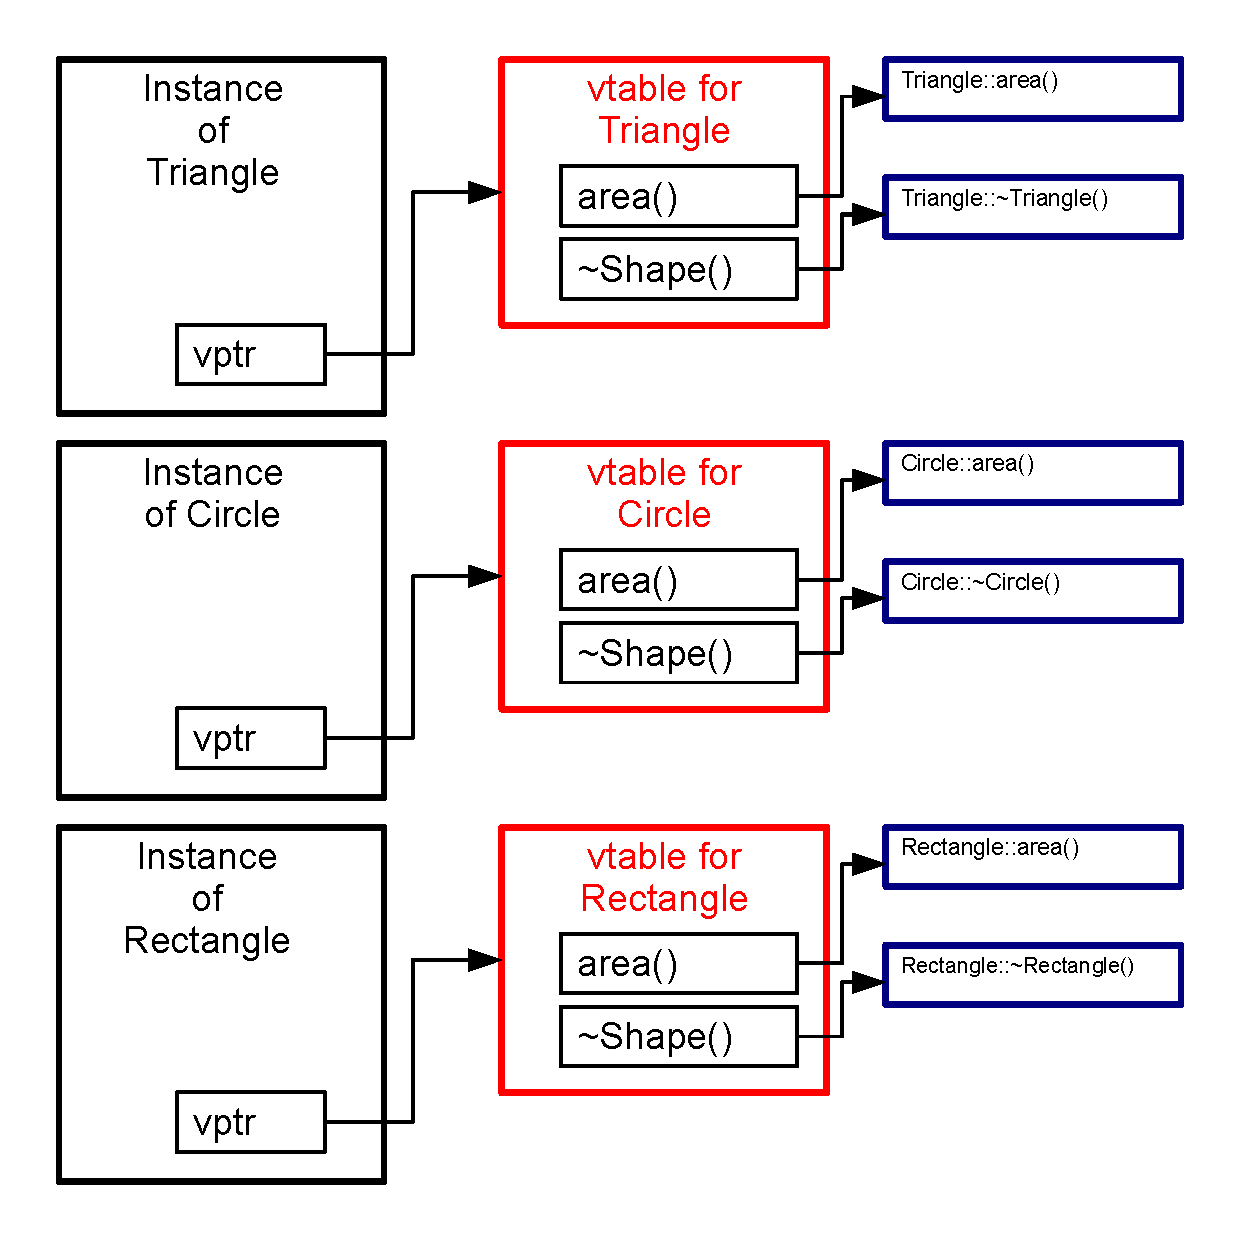
\includegraphics[width=0.8\textwidth]{vdispatch}
\caption[Virtual function dispatch]{\label{virtual_dispatch}Virtual function dispatch. Instances of classes have a pointer to the vtable for their type, which in turn holds pointers to the function definitions themselves.}
\end{figure}

The mechanism which allows virtual functions to exist is fairly complicated, and introduces some \emph{runtime overhead} over and above the usual function call mechanism.

The usual implementation (though not specified by the standard, so some implementations may use a different approach) is to add a hidden pointer called a \emph{vpointer} (virtual table pointer) to each object which has virtual functions. This pointer points to the \emph{vtable} (virtual function table) for the object. The \verb|vtable| contains pointers to the functions themselves. There is one vtable per class (that is, one providing a list of function pointers for \verb|Triangle|, one for \verb|Circle| and one for \verb|Rectangle|). The objects each hold a vpointer which is set in the constructor (by the compiler) to point to the correct vtable.

When the runtime environment hits a virtual function call, it first dereferences the object's vpointer to obtain the correct vtable, which it uses to look up the correct function to eventually call. This involves two levels of indirection (dereferencing of two pointers; the vpointer and a pointer in the vtable) before the correct function address is determined and code execution can continue. This introduces substantial runtime overhead compared to static dispatch, where the address of the function can be determined at compile time. Figure \ref{virtual_dispatch} illustrates this.

For this reason, virtual dispatch should be used only when necessary. Making a single member function virtual results in one vtable \emph{per class} and one vpointer \emph{per object}, which introduces a memory overhead as well as the runtime overhead when that virtual function is called (of course, once you already have a virtual function, adding more only increases the size of the vtable!)

\section{Overloading \& overriding}
In C++, functions can be \emph{overloaded}; that is, multiple versions of a function name can exist as long as they differ in the number or type (or both!) of their arguments (note that return types don't count for overloads; differences must be in the arguments). We've seen several examples of overloading during the course, and I talk about it in the day 2 notes as well.

\subsection{Overriding (virtual) member functions}
In a class hierarchy involving virtual member functions, there is a related concept: that of \emph{overriding}. You do this whenever you implement a virtual function in a derived class (i.e. you override the implementation from the base class with the implementation in your derived class). This is not the same as overloading, since with overloads both versions are available, but with overrides you only get the derived version (assuming you have a pointer to an object of the correct type!) What you're doing is providing a new function body for the same function signature; contrast this with overloading, where you're providing a different function signature and (possibly) different function body.

In the example below, we provide a function \verb|speak()| in the base class \emph{Animal}, and \emph{override} it in the derived classes \verb|Cat| and \verb|Dog|.
\begin{verbatim}
class Animal {
  public:
    virtual void speak()
    {
      std::cout << "I am a nondescript Animal!\n";
    }
};

class Cat : public Animal {
  public:
    virtual void speak()
    {
      std::cout << "I am a highly intelligent cat! Feed me! Meow!\n";
    }
};

class Dog : public Animal {
  public:
    virtual void speak()
    {
      std::cout << "I'm a dumb dog. Oh look, a stick. Woof!\n";
    }
};

int main()
{
  Animal* schrodinger = new Cat;
  schrodinger->speak();
  return 0;
}
\end{verbatim}

In the main function the call to \verb|schrodinger->speak()| is absolutely unambiguous. The object has dynamic type \verb|Cat|, so we get \verb|Cat::speak()|. This is the main difference between overloading and overriding. When we override, we still only have one option. If we overloaded, we'd have versions of \verb|Cat::speak()| that took different numbers or types of arguments, and the compiler would choose one based on the number and type of arguments when the function call is made. When we override, the signatures are identical and the runtime environment chooses which function to call based on the dynamic type of the object.

You can override non-virtual member functions too, but you probably shouldn't! The main reason not to do this is that you shouldn't really have implementations in your base class anyway (the example above was for illustration only), and another reason is that if someone calls your function through a pointer to base, you won't get virtual dispatch on a non-virtual function, so you get the base version anyway!

\subsection{Hiding of member functions}
Consider the class hierarchy below. In \verb|Base| we define a function \verb|func| that takes an integer argument. In \verb|Derived|, we want to be able to deal with \verb|double| arguments too, so we try to write something like this:
\begin{verbatim}
class Base {
  public:
    void func(int x); // doesn't matter if this is virtual or not
};

class Derived : public Base {
  public:
    void func(double x);
};
\end{verbatim}

We might expect this to work; that is, our derived class should have the overloaded functions \texttt{void func(int x)} and {void func(double x)}. The compiler, however, has other ideas, and will typically warn you that ``Derived::func(double) hides Base::func(int)''.

By defining a function named \verb|func| in the derived class, we hide any functions of the same name from the base class. In order to bring those into the scope of the derived class, we need a \emph{using declaration}:
\begin{verbatim}
class Base {
  public:
    void func(int x); // doesn't matter if this is virtual or not
};

class Derived : public Base {
  public:
    void func(double x);
    using Base::func; // unhides Base::func(int x)
};
\end{verbatim}

Now, we have both overloads available in the class. You may have seen this happen when you tried to implement the virtual functions from the base class \verb|EventGenerator| if you gave the function in the derived class \verb|TwoBodyEventGenerator| a different signature (different number or type of arguments, or missed off the final \verb|const| qualifier). The important thing is that \emph{when you override a virtual function the signatures must match exactly}.

Hiding occurs whenever you give a function in a derived class the same name as one in a base. You can add \emph{using declarations} to bring the names from the base class into the scope of the derived class. Note that hiding takes place when you have a (pointer to) derived object. If you have a base object (or a pointer to one) then nothing is hidden because the compiler cannot assume anything about the derived classes\footnote{See \url{http://www.parashift.com/c++-faq-lite/strange-inheritance.html\#faq-23.9} for this example in more detail.}!

\section{Functions, function pointers \& function objects}
\subsection{Functions \& function pointers}
A function name acts like a pointer to that function. This is why things like the following example work.
\begin{verbatim}
double interval(const Particle& p)
{
  return p.getFourMomentum().interval();
}

// ...

std::vector<Particle> mu_plus = fill_particle_vector("mu+");
std::vector<double> inv_masses
std::transform(mu_plus.begin(), mu_plus.end(),
               std::back_inserter(inv_masses),
               interval);
\end{verbatim}

The \verb|std::transform()| algorithm expects its final argument to be some \emph{callable} entity. A function name suffices here because it acts like a pointer to that function, which \verb|std::transform()| can ultimately call, once for each element in the range.

\subsubsection{Pointers to functions}
Like (almost) every other entity in C++, a function pointer has a well-defined type. The type of a function pointer looks a little strange, but the general form is as follows:
\begin{verbatim}
return_type (*)(argument_typelist)
\end{verbatim}

If you want to declare an object which is a function pointer, you must give the type as well as the name. What is slightly unusual is that the name goes after the \verb|*|. In the following example, we declare a few functions, as well as named function pointers which we initialise to point to those functions.

\begin{verbatim}
void printHelp(); 
void (*ptr_to_help_function)() = &printHelp;

double calculateInvariantMass(const Particle& a,
    const Particle& b);
double (*ptr_to_invmass_calc)(const Particle&,
    const Particle&) = &calculateInvariantMass;

void swapWithTmp(int& a, int& b);
void swapWithXor(int& a, int& b);
void (*my_swap_choice)(int&, int&) = &swapWithTmp;
// ...
// later:
my_swap_choice = &swapWithXor;
\end{verbatim}

Because we're initialising a pointer, we use the address-of (\verb|&|) operator before the original function name, on the right-hand side of the \verb|=| operator. On most compilers, you can get away without using the address-of operator, and just write the function name directly. Strictly speaking, we should have used the address-of operator in the \texttt{std::transform} example earlier, too!

You may wonder why we'd ever bother with creating a pointer to a function when we can just call the function directly. The reason is that it allows us to choose, at runtime, which particular function gets called. You'll notice this sounds a bit like virtual dispatch in class hierarchies; that's because it is (see section \ref{sec:vdispatch} for details on how virtual functions are usually implemented). We can use a function pointer to choose, at runtime, one of several functions to run, based on the value of some user input. For example, we could implement some of the calculator program from the first day in this manner:

\begin{verbatim}
#include <cstdlib>
#include <iostream>

double add(double a, double b) { return a + b; }
double sub(double a, double b) { return a - b; }
double mul(double a, double b) { return a * b; }
double div(double a, double b) { return a / b; }

int main()
{
  // variables to hold input from user
  char op('\0');
  double a(0.0), b(0.0);
  // function pointer to choose current
  // operation (init. to null ptr)
  double (*current_operation)(double, double) = 0;

  while ( true )
  {
    std::cout << "Enter two numbers: ";
    std::cin >> a >> b;
    std::cout << "Enter operation: [+-*/q]";
    std::cin >> op;
    switch( op )
    {
      case '+':
        current_operation = &add;
        break;
      case '-':
        current_operation = &sub;
        break;
      case '*':
        current_operation = &mul;
        break;
      case '/':
        current_operation = &div;
        break;
      case 'q':
        // quit program
        exit(0);
      default:
        // No sensible choice
        // reset to null pointer
        current_operation = 0;
        break;
    }

    // call function pointed to
    // if pointer is non-null
    if ( current_operation )
    {
      std::cout << "Answer: "
        << current_operation(a, b) << "\n";
    }
  }
  return 0;
}
\end{verbatim}

I've omitted various forms of error checking (such as testing for sensible user input, or division by zero) for the sake of clarity. What we do here is read two numbers, then decide based on user input which function to call by setting a function pointer to the address of the relevant function. The advantage we gain is that we can then call the function later, at our convenience. In this trivial example we don't really care where we called the function, but hopefully it should be obvious that this ability to make a decision about which function to call, but delay the actual calling, comes in useful.

\subsubsection{Callbacks}
One of the most common uses for function pointers is to implement \emph{callbacks}. In a callback, you give something a pointer to a function that it will call later. In this way, you can customise the behaviour of a function by providing it a different callback. The \texttt{std::transform} algorithm works in this way; you customise precisely how it transforms a sequence by giving it a callback, which it applies in turn to each element, in order to generate the output elements. Menu systems in graphical interfaces are often implemented using callbacks; each entry in the menu is represented by an object which stores a function pointer. When it is clicked, the button code calls whatever function lies at the other end of that pointer. In this way, a single menu system can be used for menus with dramatically different functionality. All you have to do is tell it the string to display in the menu it finally renders, and the function to call when someone clicks it!

Note that you can also store function pointers as the \emph{value type} in a \texttt{std::map}, so you could look up based on some key (string, integer, whatever) and call the function which was mapped to that key!

\subsection{Pointers to member functions}
The discussion in the previous section applies equally to C and C++. Functions, and function pointers, behave in the same way for both languages. C++, however, introduces classes, and with them, member functions. If you can have a member function, you should be able to have a pointer to a member function---and, indeed, you can!

If you thought the syntax for declaring a function pointer was strange, the syntax for working with pointers to member functions is stranger still. Actually, the type is fairly straightforward. If a pointer to an ordinary function looked something like:
\begin{verbatim}
return_type (*ptr_name)(argument_typelist);
\end{verbatim}
then a pointer to a member function of class Foo looks like:
\begin{verbatim}
return_type (Foo::*ptr_name)(argument_typelist);
\end{verbatim}
There's an additional caveat here; you can also have pointers to \emph{const member functions}:
\begin{verbatim}
return_type (Foo::*ptr_name)(argument_typelist) const;
\end{verbatim}

So far, so good. Nothing looks particularly different yet! We had to give the class name, and use the scope resolution operator (and this has to be done before the \verb|*| symbol), but things look pretty much as they did for ordinary function pointers.

The problem is that when you call a member function, you have to have an object associated with it! You can't call a class member function without an object for it to act on. The mechanism for specifying the object uses perhaps the most unusual operator you'll ever encounter in C++, namely \verb|.*| and \verb|->*|

The code sample below shows how this works for a class with two member functions having the same signature, using function pointers to call both member functions on objects and pointers to objects!
\begin{verbatim}
#include <cmath>
#include <iostream>

class Vector
{
  public:
    Vector(double p1x, double p1y, double p2x, double p2y)
      : x1(p1x), y1(p1y), x2(p2x), y2(p2y) {}

    double euclideanLength() const
    {
      // normal vector length
      return sqrt((x2-x1)*(x2-x1) + (y2-y1)*(y2-y1));
    }

    double manhattanLength() const
    {
      // length if you can only move in
      // straight lines on a square grid
      return (x2-x1) + (y2 - y1);
    }

  private:
    double x1;
    double y1;

    double x2;
    double y2;
};

int main()
{
  // typedefs work with function pointers
  // The typedef name also goes after the *
  typedef double (Vector::*VectFnPtr)() const;
  
  // Ask user which length measure they want
  int metric_choice(0);
  std::cout << "Enter metric choice (0, 1):";
  std::cin >> metric_choice;

  // Initialise function pointer
  // based on user choice
  VectFnPtr length_fn = 0;
  if ( metric_choice == 1 )
  {
    length_fn = &Vector::manhattanLength;
  }
  else
  {
    length_fn = &Vector::euclideanLength;
  }

  // Create a Vector
  Vector v1(0, 0, 1, 1);

  // Call whichever length function was
  // requested, and print the result
  double length_result = (v1.*length_fn)();
  std::cout << "Length: " << length_result << "\n";

  // Now allocate a Vector dynamically
  Vector* v2 = new Vector(0, 0, 2, 2);
  // Force use of manhattan length
  length_fn = &Vector::manhattanLength;
  length_result = (v2->*length_fn)();
  std::cout << "Manhattan length (expect 4): "
    << length_result << "\n";
  
  return 0;
}
\end{verbatim}

Everything looks fine until we hit the point where we want to call the member functions. If we have an object (or reference to an object) we first associate the member function with the object by dereferencing it (with \verb|*|) and using the member access operator (\verb|.|); then we call the function using \emph{function call brackets}---arguments, if any, would go inside these brackets:
\begin{verbatim}
result = (obj.*ptr)(arg, ...);
\end{verbatim}

This sort of makes sense. If a function pointer \texttt{ptr} holds the address of a function, then \verb|*ptr| is the function itself. Since we could normally do \verb|obj.member|, we can now do \verb|obj.*ptr|. The extra brackets are needed to get around the rules C++ has for precedence of operators; you first need to give the function pointer an object to work on, then you call it. The first set of brackets in the call construct the object--member-function pair, while the second set actually call it! If you wanted to give a member function arguments, you'd do something like:
\begin{verbatim}
class A {
  public:
    double square(double x) { return x*x; }
};

// elsewhere
double (A::*func_ptr)(double) = &A::square;
A my_a;
double result = (my_a.*func_ptr)(3.14);
\end{verbatim}

Obviously, if you have a pointer to an object, you use \verb|->| instead of \verb|.| so the whole thing looks like:
\begin{verbatim}
class A {
  public:
    double square(double x) { return x*x; }
};

// elsewhere
double (A::*func_ptr)(double) = &A::square;
A* my_a_ptr = new A;
double result = (my_a_ptr->*func_ptr)(3.14);
\end{verbatim}

Pointers to member functions actually aren't used all that often. Mostly, this is because virtual dispatch and public inheritance solve a lot of the problems for which we'd want to use pointers to member functions. The compiler will typically use pointers to member functions behind the scenes, in order to implement virtual dispatch, but you don't have to worry about that! One final note is that if you're within a class member function already, you can use \verb|this| as a pointer to the object (as per usual) in association with a pointer to member function. I'm sure you can figure out the syntax for that, by now!

\subsection{Function objects (functors)}
The other reason that you rarely need pointers to member functions is that you can define \verb|operator()| for a class. This is the \emph{function call operator} (also called \emph{operator brackets} or \emph{operator paren-paren}). Doing this makes the object a function object, or a functor.

Functors can be called just like normal functions, only this time the name is an object, not a function! That is, you write the name of the object followed by function call brackets, into which you write any arguments that \verb|operator()| takes. An example follows, of course.

\begin{verbatim}
#include <algorithm>
#include <iterator>
#include <iostream>
#include <vector>

class Power {
  public:
    explicit Power(int pow)
      : N(pow) {}

    int operator()(int i)
    {
      int result(i);
      for (int j = 1; j < N; ++j)
      {
        result *= i;
      }
      return result;
    }

  private:
    int N;
};

int main()
{
  // input vector
  // contains numbers 1, 2, 3
  std::vector<int> input(3);
  input[0] = 1;
  input[1] = 2;
  input[2] = 3;

  // Create a functor which gives 
  // us the 4th power of a number
  Power quad(4);
  // and use it directly on the value 2
  std::cout << quad(2) << "\n";

  // Use the same functor as the unary operator
  // in a call to std::transform()
  std::transform(input.begin(),
      input.end(),
      std::ostream_iterator<int>(std::cout, " "),
      quad);
  std::cout << "\n";

  // And this time create a temporary Power object
  // to pass as an argument to std::transform()
  // (This time, we get the 8th power)
  std::transform(input.begin(),
      input.end(),
      std::ostream_iterator<int>(std::cout, " "),
      Power(8));
  std::cout << "\n";

  return 0;
}
\end{verbatim}

The output is as follows:
\begin{verbatim}
16
1 16 81 
1 256 6561
\end{verbatim}

We can use a functor any time we want to make a function call depend on some additional state. In this case, that state is the power to which to raise an argument. We could have stored a second vector whose elements are all $4$, and used the version of \verb|std::transform()| with a binary operator and two input sequences, but that's a lot of overhead, and it's hard to change to give the 8th power. In the example above, we wrote a simple class that stores this additional information as a member variable, and uses it on each application of \verb|operator()|. This is much more efficient, and more easily customisable.

It is also possible to store much more complicated state, e.g. to accumulate values from a vector (but see \verb|std::accumulate()| for a better way to do this!)

\section{Static class members}
In day 5 you saw the \emph{singleton} design pattern used to implement the \verb|ParticleInfo| class. In this class, we used \emph{static member functions} and a \emph{static member variable}.

\subsection{Static member functions}
A static member function (sometimes called a \emph{class method}) is a function within the scope of the class that can be called without an instance of that class. In other words, you don't have to create an object of that class in order to call a static member function. We use this in the \verb|ParticleInfo| singleton to control creation of (and access to) \verb|ParticleInfo| objects. The \verb|ParticleInfo::Instance()| member function is declared static, so that users can call it without already having access to a \verb|ParticleInfo| object. This is, obviously, necessary because calling this function is the \emph{only} way they can get access to a \verb|ParticleInfo| object!

Static member functions should be used sparingly. They are essential for implementing the singleton design pattern (which should, itself, be used sparingly) but otherwise they are typically an indication that your design is flawed.

\subsection{Static member variables}
Static member variables are variables within class scope that have \emph{just one instance} which is \emph{shared between all objects of that class}. Examples from this course include the variables \verb|FourVector::c| and \verb|FourVector::c2| which are defined to be the speed of light and the speed of light squared, respectively. This information is used within the \verb|FourVector| class to compute Lorentz boosts and space-time intervals, but we don't need to give each \emph{object} a copy; the speed of light doesn't change, and it doesn't make much sense to have multiple copies of a single constant floating around, so we chose to make this variable a class static member variable. Another example is the value \verb|ThreeVector::Pi|, which represents the value of $\pi$. We only need one copy of this, and all \verb|ThreeVector| objects can access it.

You should be able to see a theme emerging here; static member variables (especially const ones) are useful for representing constants within some enclosing scope. This is a much better approach than using global variables---but beware of using one static variable to initialise another; the rules for initialisation of static variables are complicated and the order of initialisation across translation units (roughly, source code files) is not well defined.

In the \verb|ParticleInfo| singleton, we saw another example of a static member variable. This time, it was a pointer to the single instance of \verb|ParticleInfo|. The reason that this must be static is that you access an instance by calling the static \verb|ParticleInfo::Instance()| member function. A static member function can only access static member variables, so the \verb|ParticleInfo* theInstance| must be static too.

Singletons go some way towards solving the problem of static initialisation, because they are guaranteed to be initialised by the time \verb|Instance()| returns. For this reason, some people overuse singletons to represent almost any global (ish) constant variable. Global variables are very bad, and while singletons are better, they are not much better. It is usually best to change the design to avoid global objects altogether!

\section{Further reading}
Rather than making this document even longer than it already is by including details of many more advanced features of C++, I present here a list of resources, grouped broadly by category (with some duplication), for those who wish to go further.

\subsection{C++ language \& library features}
The following are considered introductory or intermediate C++ texts. They cover features of the language itself and of the standard library.

\begin{itemize}
	\item The C++ Programming Language, (Special) 3rd Edition, \emph{Bjarne Stroustrup}, Addison Wesley, 2000. A comprehensive introduction and reference for the C++ language and library. Written by the creator of C++.
	\item Accelerated C++, \emph{Andrew Koenig \& Barbara E. Moo}, Addison Wesley, 2000. A more approachable introduction to C++, aimed at getting you quickly writing software using most of the features of C++. This is the same Koenig as Koenig lookup (Argument dependent lookup).
	\item The C++ Standard Library: A tutorial and reference, \emph{Nicolai M. Josuttis}, Addison Wesley, 1999. A tour of the standard library. Covers containers, algorithms, iterators, adapters and binders.
\end{itemize}

\subsection{Improving your use of C++}
The following books provide lists of specific features of C++ that can improve your programming. They should be read from cover to cover at least once, and consulted regularly!

\begin{itemize}
	\item Effective C++ (Third Edition): 55 specific ways to improve your programs and designs, \emph{Scott Meyers}, Addison Wesley, 2005. A list of specific aspects of C++ that you can start using immediately to improve your programs.
	\item More Effective C++: 35 new ways to improve your programs and designs, \emph{Scott Meyers}, Addison Wesley, 1995. A few more ways you can improve your use of the C++ language features.
	\item Effective STL: 50 specific ways to improve the use of the standard template library, \emph{Scott Meyers}, Addison Wesley, 2001. Targets the standard library and shows you how you can improve the way you write C++ programs using it.
	\item Exceptional C++, \emph{Herb Sutter}, Addison Wesley, 1999. This book poses a number of problems in C++ and explains how the expected behaviour of C++ isn't always what you get. Demonstrates the boundary cases in C++ and pushes the limits!
	\item More Exceptional C++, \emph{Herb Sutter}, Addison Wesley, 2001. More problems, solutions, boundary cases. Some discussion of exception safety, which might be worth reading if your projects use exceptions!
\end{itemize}

\subsection{Templates}
The following books deal with the topic of templates in some considerable detail.

\begin{itemize}
	\item C++ Templates: The Complete Guide, \emph{David Vandevoorde \& Nicolai M. Josuttis}, Addison Wesley, 2002. Comprehensive text covering almsot all of the aspects of C++ templates and generic programming.
	\item C++ Template Metaprogramming: Concepts, Tools and Techniques from Boost and Beyond, \emph{David Abrahams \& Aleksey Gurtovoy}, Addison Wesley, 2004. A detailed look at template metaprogramming, the use of templates to do useful work at compile time!
\end{itemize}

\subsection{Boost}
The following books describe the Boost libraries, some of which are now part of the C++11 (ISO/IEC 14882:2011) standard.

\begin{itemize}
	\item Beyond the C++ Standard Library: An Introduction to Boost, \emph{Bjorn Karlsson}, Addison Wesley, 2005. Introduces many of the Boost libraries and provides detailed examples of their use.
	\item The Boost C++ Libraries, \emph{Boris Schaling}, XML Press (2011). A more in-depth look at the Boost libraries, including some of the more obscure applications of template metaprogramming (e.g. the Boost.Spirit parser framework).
	\item C++ Template Metaprogramming: Concepts, Tools and Techniques from Boost and Beyond, \emph{David Abrahams \& Aleksey Gurtovoy}, Addison Wesley, 2004. A detailed look at template metaprogramming, the use of templates to do useful work at compile time!
\end{itemize}

\subsection{Design Patterns}
The following books deal with recurring themes in C++ systems and some of the patterns that have emerged for them.

\begin{itemize}
	\item Design Patterns: Elements of reusable object-oriented software, \emph{Erich Gamma, Richard Helm, Ralph Johnson \& John Vlissides}, Addison Wesley, 1994. Old, but still incredibly relevant. This book should be your first port of call when implementing many common patterns. The so-called ``Gang of Four'' (GoF) book.
	\item Modern C++ Design, \emph{Andrei Alexandrescu}, Addison Wesley, 2001. An in-depth look at the issues surrounding many design issues in C++; design patterns, their implementations, and their limitations. Focuses strongly on templates, policy-based design and generic programming.
\end{itemize}

\subsection{Standards}
The definitive source of information on C++. While most textbooks will give you the usual behaviour, the standard is the precise specification of how C++ behaves in every circumstance.

\begin{itemize}
	\item The C Standard, \emph{British Standards Institute}, Wiley, 2003. The definition of ISO/IEC 9899:1999 (The C Programming Language).
	\item The C++ Standard, \emph{British Standards Institute}, Wiley, 2003. The definition of ISO/IEC 14882:2003 (The C++ Programming Language).
	\item JTC1/SC22/WG21 - The C++ Standards Committee, \url{http://open-std.org/JTC1/SC22/WG21/}. Public draft releases of the C++ 2011 standard (ISO/IEC 14882:2011) and additional material.
\end{itemize}

\end{document}
